\documentclass[
ngerman,
twoside,
pdfa=false,
ruledheaders=section,%Ebene bis zu der die Überschriften mit Linien abgetrennt werden, vgl. DEMO-TUDaPub
class=report,% Basisdokumentenklasse. Wählt die Korrespondierende KOMA-Script Klasse
thesis={type=sta},% Dokumententyp Thesis, für Dissertationen siehe die Demo-Datei DEMO-TUDaPhd
accentcolor=TUDa-2c,% Auswahl der Akzentfarbe
custommargins=false,% Ränder werden mithilfe von typearea automatisch berechnet
marginpar=false,% Kopfzeile und Fußzeile erstrecken sich nicht über die Randnotizspalte
%BCOR=5mm,%Bindekorrektur, falls notwendig
parskip=half-,%Absatzkennzeichnung durch Abstand vgl. KOMA-Sript
fontsize=11pt,%Basisschriftgröße laut Corporate Design ist mit 9pt häufig zu klein
%	logofile=tuda_logo.pdf, %Falls die Logo Dateien nicht installiert sind
]{tudapub}

%%%%%%%%%%%%%%%%%%%%%%%%%%%%
% Download des TU-Logos
%%%%%%%%%%%%%%%%%%%%%%%%%%%%
% https://download.hrz.tu-darmstadt.de/protected/CE/TUDa_LaTeX/tuda_logo.pdf
% Der Pfad zum Logo kann als "logofile" angegeben werden.

%%%%%%%%%%%%%%%%%%%
% Sprachanpassung & Verbesserte Trennregeln
%%%%%%%%%%%%%%%%%%%
\usepackage[english, main=ngerman]{babel}
\usepackage[autostyle]{csquotes}% Anführungszeichen vereinfacht
\usepackage{microtype}

%%%%%%%%%%%%%%%%%%%
% Literaturverzeichnis
%%%%%%%%%%%%%%%%%%%
\usepackage{biblatex}   % Literaturverzeichnis
\addbibresource{HausarbeitBib.bib}

%%%%%%%%%%%%%%%%%%%
% Paketvorschläge Tabellen
%%%%%%%%%%%%%%%%%%%
%\usepackage{array}     % Basispaket für Tabellenkonfiguration, wird von den folgenden automatisch geladen
\usepackage{tabularx}   % Tabellen, die sich automatisch der Breite anpassen
%\usepackage{longtable} % Mehrseitige Tabellen
%\usepackage{xltabular} % Mehrseitige Tabellen mit anpassarer Breite
\usepackage{booktabs}   % Verbesserte Möglichkeiten für Tabellenlayout über horizontale Linien

%%%%%%%%%%%%%%%%%%%
% Paketvorschläge Mathematik
%%%%%%%%%%%%%%%%%%%
\usepackage{mathtools} % erweiterte Fassung von amsmath
\usepackage{amssymb}   % erweiterter Zeichensatz
\usepackage[decimalsymbol=comma]{siunitx}   % Einheiten
\usepackage{amsmath}


%%%%%%%%%%%%%%%%%
% Eigenen Pakete Gruppe01
%%%%%%%%%%%%%%%%%%%%
%\usepackage[utf8]{inputenc}
%\usepackage[ngerman]{babel}
\usepackage{hyperref}
\usepackage{graphicx}
\usepackage{subcaption}
\usepackage{listings}
\usepackage[framed, numbered]{matlab-prettifier}
%\usepackage[style=numeric]{biblatex}
%\usepackage{amsthm}
%\usepackage[squaren]{SIunits}
\usepackage{enumitem}
\usepackage{tikz}
\usepackage{pgfplots}
\usepackage{pgfplotstable}
%\usepackage{booktabs}
\pgfplotsset{compat=1.12}
\usepackage{dsfont}
\usepackage{arcs}

\usepackage{media9}

%%%%%%%%%%%%%%%%%%%
% verschiedene Nummerierung für Abbildungen und Formeln
%%%%%%%%%%%%%%%%%%%
\usepackage{chngcntr}
%\counterwithout{equation}{chapter}


%%%%%%%%%%%%%%%%%%%
% Pseudocode
%%%%%%%%%%%%%%%%%%%
\usepackage[linesnumbered,lined,boxruled]{algorithm2e} % Package für Pseudocode

%%%%%%%%%%%%%%%%%%%
% Plotting und Grafik
%%%%%%%%%%%%%%%%%%%
\usepackage{tuda-pgfplots} % Package für Plotting with TUDa mods

%%%%%%%%%%%%%%%%%%%
% Sonstiges
%%%%%%%%%%%%%%%%%%%
\usepackage{blindtext} % Package für Blindtext

\renewcommand{\tt}[1]{\texttt{#1}} 
\newcommand{\m}[1]{\textrm{#1}} 
\renewcommand{\b}[1]{\textbf{#1}} 
\newcommand{\mb}[1]{\mathbf{#1}} 


\begin{document}
	
	\title{Ausarbeitung Übung 8}
	%\subtitle{Ein Untertitel, wenn nötig}
	\author[D. Schiller, C. Kramer, S.Arnold, T. Lingenberg]{Dominik Schiller \and Constanze Kramer \and Simon Arnold \and Tobias Lingenberg} %optionales Argument ist die Signatur,
	%\reviewer{Gutachter 1 \and Gutachterin 2} %Gutachten
	
	%Diese Felder werden untereinander auf der Titelseite platziert.
	\department{} % Das Kürzel wird automatisch ersetzt und als Studienfach gewählt, siehe Liste der Kürzel im Dokument.

	
	\date{\today}
	%\examdate{\today}
	
	%	\tuprints{urn=1234,printid=12345}
	%	\dedication{Für alle, die \TeX{} nutzen.}
	
	\maketitle
	\pagenumbering{gobble} % Seitenzahlen angezeigt, startet ab dem Inhaltsverzeichnis
	
	
	%\affidavit
	%\AffidavitSignature
	%\AffidavitSignature
	
	
	%%%%%%%%%%%%%%%%%%%
	%Abstract / Kurzzusammenfassung
	%%%%%%%%%%%%%%%%%%%
	%\include{chapters/zusammenfassung}
	
	%%%%%%%%%%%%%%%%%%%
	%Inhaltsverzeichnis 
	%%%%%%%%%%%%%%%%%%%
	\cleardoublepage
	\tableofcontents % Erstellte ein Inhaltsverzeichnis
	
	%\cleardoublepage
	\pagenumbering{arabic} % Seitenzahlen angezeigt, startet ab dem Inhaltsverzeichnis
	\setcounter{page}{1} % Setzt den Seitenzahlenzähler auf 1
	
	%%%%%%%%%%%%%%%%%%%%%%%%%%%%%%%%%%%%%%%%%%%%%%%%%%%%%%%%%%%%%%%%%%%%%%%%%%%%%%%%%%%%%%%%%%%%%%%%%%
	
	% INHALT, am Besten ausgelagert in eigene Files/Kapitel und dann mit \include{Unterordner/Filename} eingefügt, sorgt für bessere Übersichtlichkeit und Fehlersuche. Einzelne Dateien sind aktuell im Ordner Sections abgelegt. 
	%%%%%%%%%%%%%%%%%%Einleitung%%%%%%%%%%%%%%%%%
	\chapter{Einleitung}\label{sec:intro}
Diese Arbeit beschäftigt sich mit dem Übungsblatt 9 des Faches \glqq Einführung in die numerische Berechnung elektromagnetischer Felder\grqq{}.
Zunächst wird der primale Divergenz und Rotationsoperator in Octave implementiert und berechnet. Anschließend wird eine Materialmatrix berechnet. Abschließend wird das Magnetfeld von zwei stromdruchflossenen Leitern in Octave simuliert. 
	%%%%%%%%%%%%%%%%%%Haupteil%%%%%%%%%%%%%%%%%%%
	\chapter{Bearbeitung der Aufgaben}
\section{Doppelwirbelgleichung in 2D und 3D}

Aus der statischen Doppelwirbelgleichung
\begin{equation}
\label{gl:dw}
\operatorname{rot}\operatorname{rot}\vec{A} = \mu\vec{J},
\end{equation}
lässt sich die skalare Laplace-Gleichung (\ref{gl:laplace})  für den 2D Fall mit $\vec{A} = [0,0,A_z]^T$ herleiten:
\begin{align*}
\operatorname{rot}\operatorname{rot}\vec{A} &= \mu\vec{J} \\
\operatorname{grad}\operatorname{div}\vec{A} - \Delta\vec{A} &= \mu\vec{J},
\end{align*}
wobei
\begin{align*}
\operatorname{grad}\operatorname{div}\vec{A} - \Delta\vec{A} = \nabla\left(\nabla \cdot [0,0,A_z]^T \right)
= \nabla (\partial_z A_z) = 0.
\end{align*}
Hierbei ist $\partial_z A_z = 0$, da $A_z$ im zweidimensionalen Fall nur von $x$ und $y$ anhängt. Damit ergibt sich schließlich die Laplace-Gleichung

\begin{equation}
\label{gl:laplace}
\Delta\vec{A} = -\mu\vec{J}
\end{equation}

Das Feld $\vec{A} = [0,0,A_z]^T$ genügt mit $\nabla \cdot \vec{A} = 0$ der Coulomb-Eichung. Daher ist $\vec{A}$ bis auf eine additive Konstante $A = [0,0,A_z+c]^T$ bestimmt.

Nun soll mithilfe des Faraday'schen Gesetzes (\ref{gl:fara}) die gedämpfte Wellengleichung (\ref{gl:welle}) hergeleitet werden. Hierfür werden die folgenden Maxwell'schen Gleichungen benötigt:

\begin{equation}
\label{gl:fara}
\operatorname{rot}\vec{E} = -\partial_t\vec{B}
\end{equation}
\begin{equation}
\label{gl:max2}
\operatorname{rot}\vec{B} = \mu_0\left(\partial_t\varepsilon_0\vec{E} + \vec{J}\right) \qquad \text{mit } \vec{J} = \sigma\vec{E}
\end{equation}
\begin{equation}
\label{gl:max3}
\operatorname{div}\vec{E} = \frac{\rho}{\varepsilon_0}
\end{equation}

Nach Anwenden des Rotationsoperators auf (\ref{gl:fara}) erhält man:

\begin{align*}
\operatorname{rot}\vec{E} &= -\partial_t\vec{B} \\
\operatorname{rot}\operatorname{rot}\vec{E} &= -\partial_t\operatorname{rot}\vec{B} \\
\operatorname{rot}\operatorname{rot}\vec{E} &= -\partial_t\mu_0(\partial_t\varepsilon_0\vec{E}+\vec{J}) \qquad \text{nach einsetzen von (\ref{gl:max2})} \\
\operatorname{grad}\operatorname{div}\vec{E} -\Delta\vec{E} &= -\partial_t\mu_0(\partial_t\varepsilon_0\vec{E}+\sigma\vec{E}) \\
\operatorname{grad}\left(\frac{\rho}{\varepsilon_0}\right) -\Delta\vec{E} &= -\partial_t\mu_0(\partial_t\varepsilon_0\vec{E}+\sigma\vec{E}) \qquad \text{nach einsetzen von (\ref{gl:max3})}\\
\end{align*}
Wir haben $\rho = 0$ gesetzt, da wir keinen anderen Weg gefunden haben den letzten störenden Term zu eliminieren. Somit gilt unsere gedämpfte Wellengleichung nur im Ladungsfreien Raum.

\begin{equation}
\label{gl:welle}
-\Delta\vec{E} + \mu_0\varepsilon_0\partial_t^2\vec{E} + \underbrace{\mu_0\partial_t(\sigma\vec{E})}_{\text{Dämpfung}} = 0
\end{equation}

Möchte man diese Formel nun mit der Potentialformulierung $\vec{E} = -\partial_t\vec{A} - \nabla\Phi$ ausdrücken erhält man:

\begin{equation}
\Delta(\partial_t\vec{A} + \nabla\Phi) - \mu_0\varepsilon_0\partial_t^2(\partial_t\vec{A} + \nabla\Phi) - \mu_0\partial_t(\sigma(\partial_t\vec{A} + \nabla\Phi)) = 0
\end{equation}

Es wird schnell deutlich, dass dieses Vorgehen nicht empfehlenswert ist. Es handelt sich, neben der Länge der Formel, nun auch um eine Differenzialgleichung dritter Ordnung, zuvor war die Ordnung nur zwei. Dies erschwert das Lösen der Gleichung erheblich.
 
	\chapter{titlsade}
\section{Geschichteter Kondensator}

Ein geschichteter Plattenkondensator lässt sich mit verschiedenen Programmen graphisch darstellen und analysieren. Während FEMM auf eine zwei Dimensionale Darstellung des Problems beschränkt ist, lassen sich mit Hilfe der Methode der Finiten Integration (FIT) und einem geeigneten Simulationsprogramm drei Dimensionale Darstellungen erzeugen. Das angehängte Skript \tt{SkriptAg8\_2} bildet den Vorgang der FIT ab, die Ergebnisse werden in ParaView graphisch dargestellt.\\ \\
Zur Berechnung wird das Gebiet $\Omega = \{-1,1\}^3$ betrachtet, es gilt $N_x = N_y = N_z = 21$ und damit $Np = 9261$, dieses Gebiet wird kanonisch nummeriert. Allgemein wird ein Plattenkondensator mit linear-variierender Permittivität nachgestellt, die unterschiedlichen Permittivitäten werden mit der Methode \tt{calc\_eps\_linear} bestimmt und in einem Vektor gespeichert. Des Weiteren ist an den Knoten, die die Elektroden widerspiegeln eine \textsc{Dirichlet}-Randbedingung vorgegeben. Das Potential an diesen Knoten beträgt jeweils \SI{0}{\volt} bzw. \SI{1}{\volt}. Das elektrische Feld und die Potentiale zwischen den beiden Elektroden gilt es zu berechnen. \\ \\
Die Methode \tt{createMeps} liefert die zur Rechnung benötigte Matrix $\mb{M}_\epsilon$, sie führt eine Materialmittlung durch. Um nun alle Potentiale in dem Gebiet $\Omega$ zu berechnen, muss das Gleichungssystem 
\begin{equation}
	\tilde{\mb{S}}\mb{M}_\epsilon\tilde{\mb{S}}^T\mb{\Phi} = 0
	\label{eq:meps}
\end{equation} berechnet werden. Zur Vereinfachung nimmt man an, dass $\mb{A} = \tilde{\mb{S}}\mb{M}_\epsilon\tilde{\mb{S}}^T$ gilt. Durch diese Rechnung wird garantiert, dass nur im Rechengebiet befindliche Gitterkanten und keine Geisterkanten beachtet werden, die Struktur der Matrix ist in Abbildung ?? zu sehen.\\ \\
In $\mb{\Phi}$ befinden sich sowohl die bekannten Potentiale der Randbedingungen, als auch die noch unbekannten Potentiale. Ist das Potential $\phi_n$ an einem Knoten $P_n$ des Gitters bekannt, so kann die $n$-te Zeile und Spalte der Matrix \b{A} gestrichen werden, sowie der $n$-te Eintrag aus dem Vektor $\mb{\Phi}$.\\
Die $n$-te Spalte, abzüglich des Eintrags in der $n$-ten Zeile, der Matrix \b{A} wird auf der anderen Seite des Gleichungssystems (\ref{eq:meps}) abgezogen und mit dem bekannten $\phi_n$ multipliziert. Führt man dies nun für alle Punkte durch, bei denen die Randbedingung bekannt ist, so entsteht ein Gleichungssystem der Form 
\begin{equation*}
	\mb{A}_{11}\mb{x}_1 = -\mb{A}_{12}\mb{x}_2,
\end{equation*} 
wobei in $\mb{x}_1$ alle nicht bekannten und in $\mb{x}_2$ alle bekannten Potentiale gespeichert sind. $\mb{x}_1$ lässt sich nun in Matlab ganz einfach mit $$\mb{x}_1 = -\mb{A}_{11}\backslash\mb{A}_{12}\mb{x}_2$$ berechnen. Der Potentialvektor $\mb{\Phi}$ kann aus $\mb{x}_1$ und $\mb{x}_2$ in der richtigen Reihenfolge bestimmt werden. Das dazugehörige elektrische Feld mit  
	\chapter
\section{Beschleunigermagnet, FEMM}

In Abbildung \ref{fig:Linear} ist der Verlauf des Magnetfeldes in einem vereinfachten Modell des Beschleunigermagnets SIS-100, der im FAIR Projekt der Gesellschaft für Schwerionenforschung verwendet wird, zu sehen. In dieser Simulation wurde ein linearer Materialzusammenhang zwischen magnetischer Flussdichte B und magnetischer Feldstärke H angenommen. Das B-Feld hat hierbei ein Maximum von ca. $\SI{5,7}{Tesla}$. Die Flusslinien sind annähernd homogen allerdings ist zu erkennen, dass in der Nähe des Luftspaltes die Flusslinien deutlich näher beieinander liegen.

\begin{figure}[h!]
	\centering
	\begin{subfigure}[h]{.28\textwidth}
		\centering
		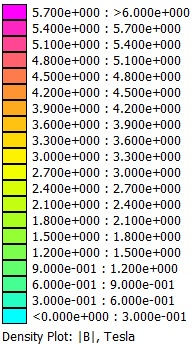
\includegraphics[width=\textwidth]{data/skala_linear}
		\caption{Skala}
		\label{fig:SkalaLin}
	\end{subfigure}
	\begin{subfigure}[h]{.60\textwidth}
		\centering
		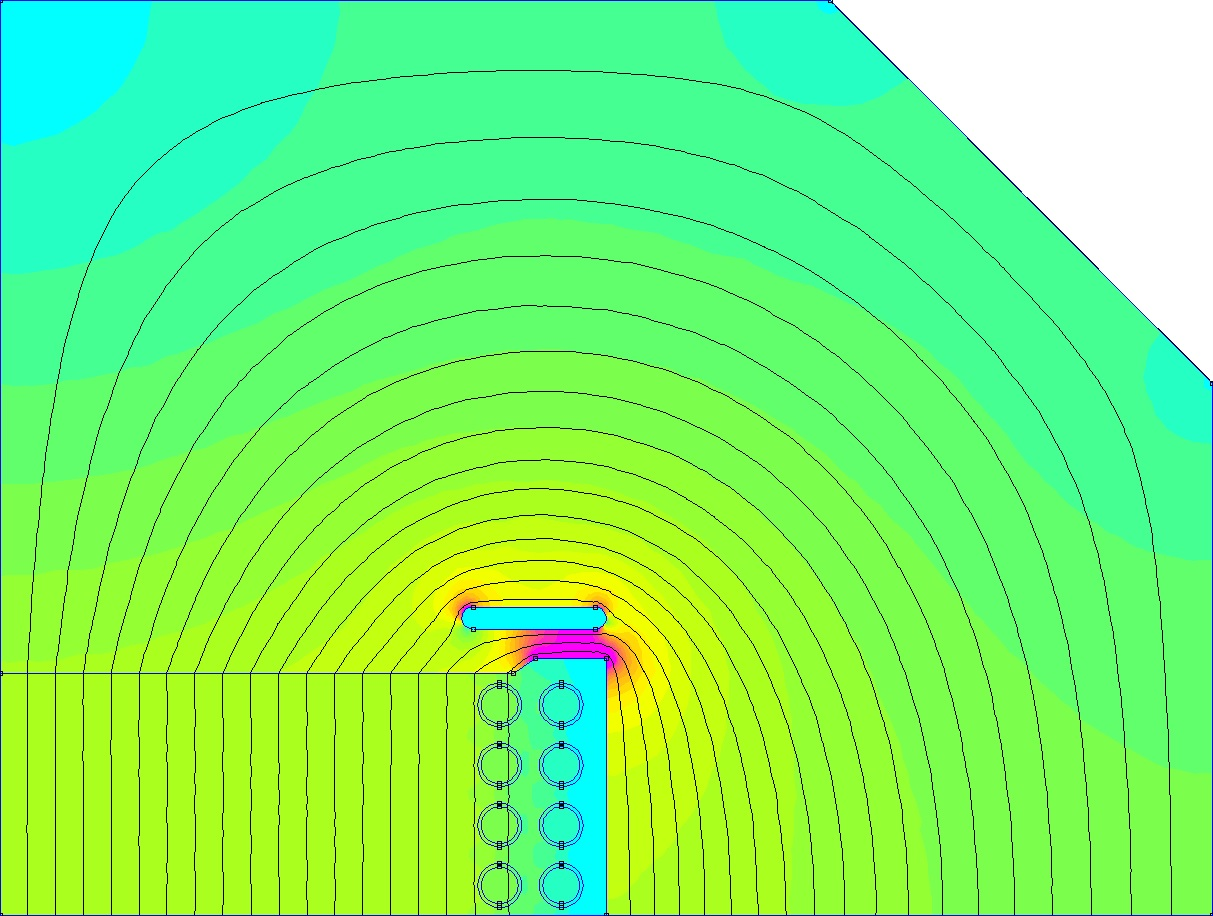
\includegraphics[width=\textwidth]{data/Linear}
		\caption{Lineare statische Simulation des Beschleunigermagnets SIS-100 in FEMM}
		\label{fig:Linear}
	\end{subfigure}	
\end{figure}

Weist man dem Eisenjoch eine nichtlineare Materialbeziehung zu ergibt sich daraus Abbildung \ref{fig:NichtLinear}. Der maximale Wert des B-Felds ist hier mit ca. $\SI{2,1}{Tesla}$ geringer als bei der linearen Simulation. Außerdem sind die Flusslinien noch deutlich homogener verteilt. Das liegt daran, dass bei dieser Simulation das Eisenjoch in Sättigung geht.

\begin{figure}[h!]
	\centering
	\begin{subfigure}[h]{.28\textwidth}
		\centering
		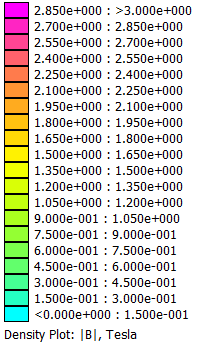
\includegraphics[width=\textwidth]{data/Skala_nichtlinear}
		\caption{Skala}
		\label{fig:SkalaNonlin}
	\end{subfigure}
	\begin{subfigure}[h]{.60\textwidth}
		\centering
		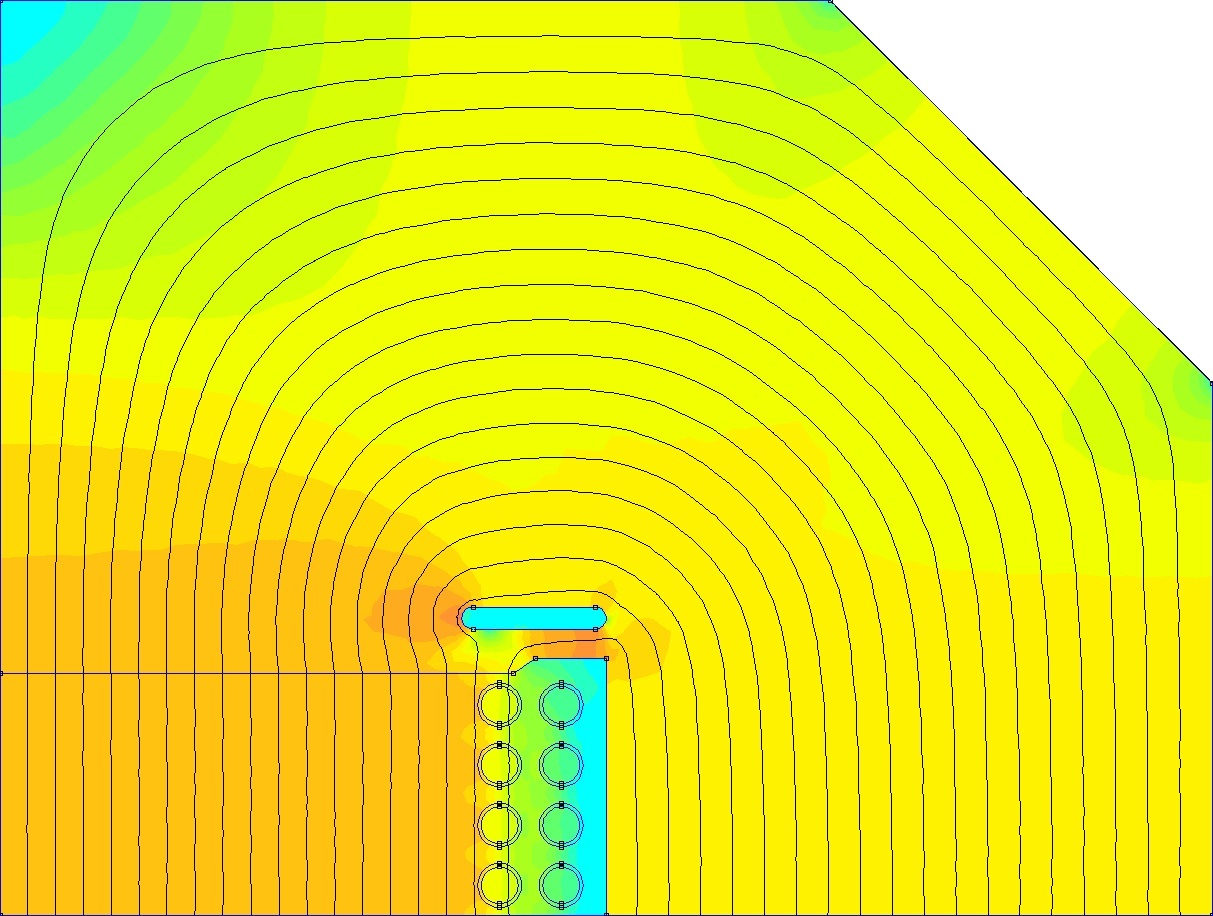
\includegraphics[width=\textwidth]{data/Nichtlinear}
		\caption{Simulation des Beschleunigermagnets SIS-100 mit nichtlinearer Materialbeziehung}
		\label{fig:NichtLinear}
	\end{subfigure}	
\end{figure}

Über die Funktion \texttt{lineintegral} lässt sich die durchschnittliche Flussdichte über einen bestimmten Bereich berechnen. Mit 

\begin{equation*}
	L = \frac{\Psi}{I}
\end{equation*}

und

\begin{equation*}
	\Psi = \int_{A} \vec{B} \mathrm{d}\vec{A}
\end{equation*}

ergibt sich die Induktivität zu

\begin{equation*}
	L = \frac{B A}{I}
\end{equation*}
 

 Wie in Abbildung \ref{fig:plot} zu sehen ist, nimmt die Induktivität kontinuierlich ab, sobald eine Stromanregung von etwa $\SI{6000}{A}$ angelegt wird da dann der Eisenkern in Sättigung geht.


\begin{figure}[h]
	\centering
	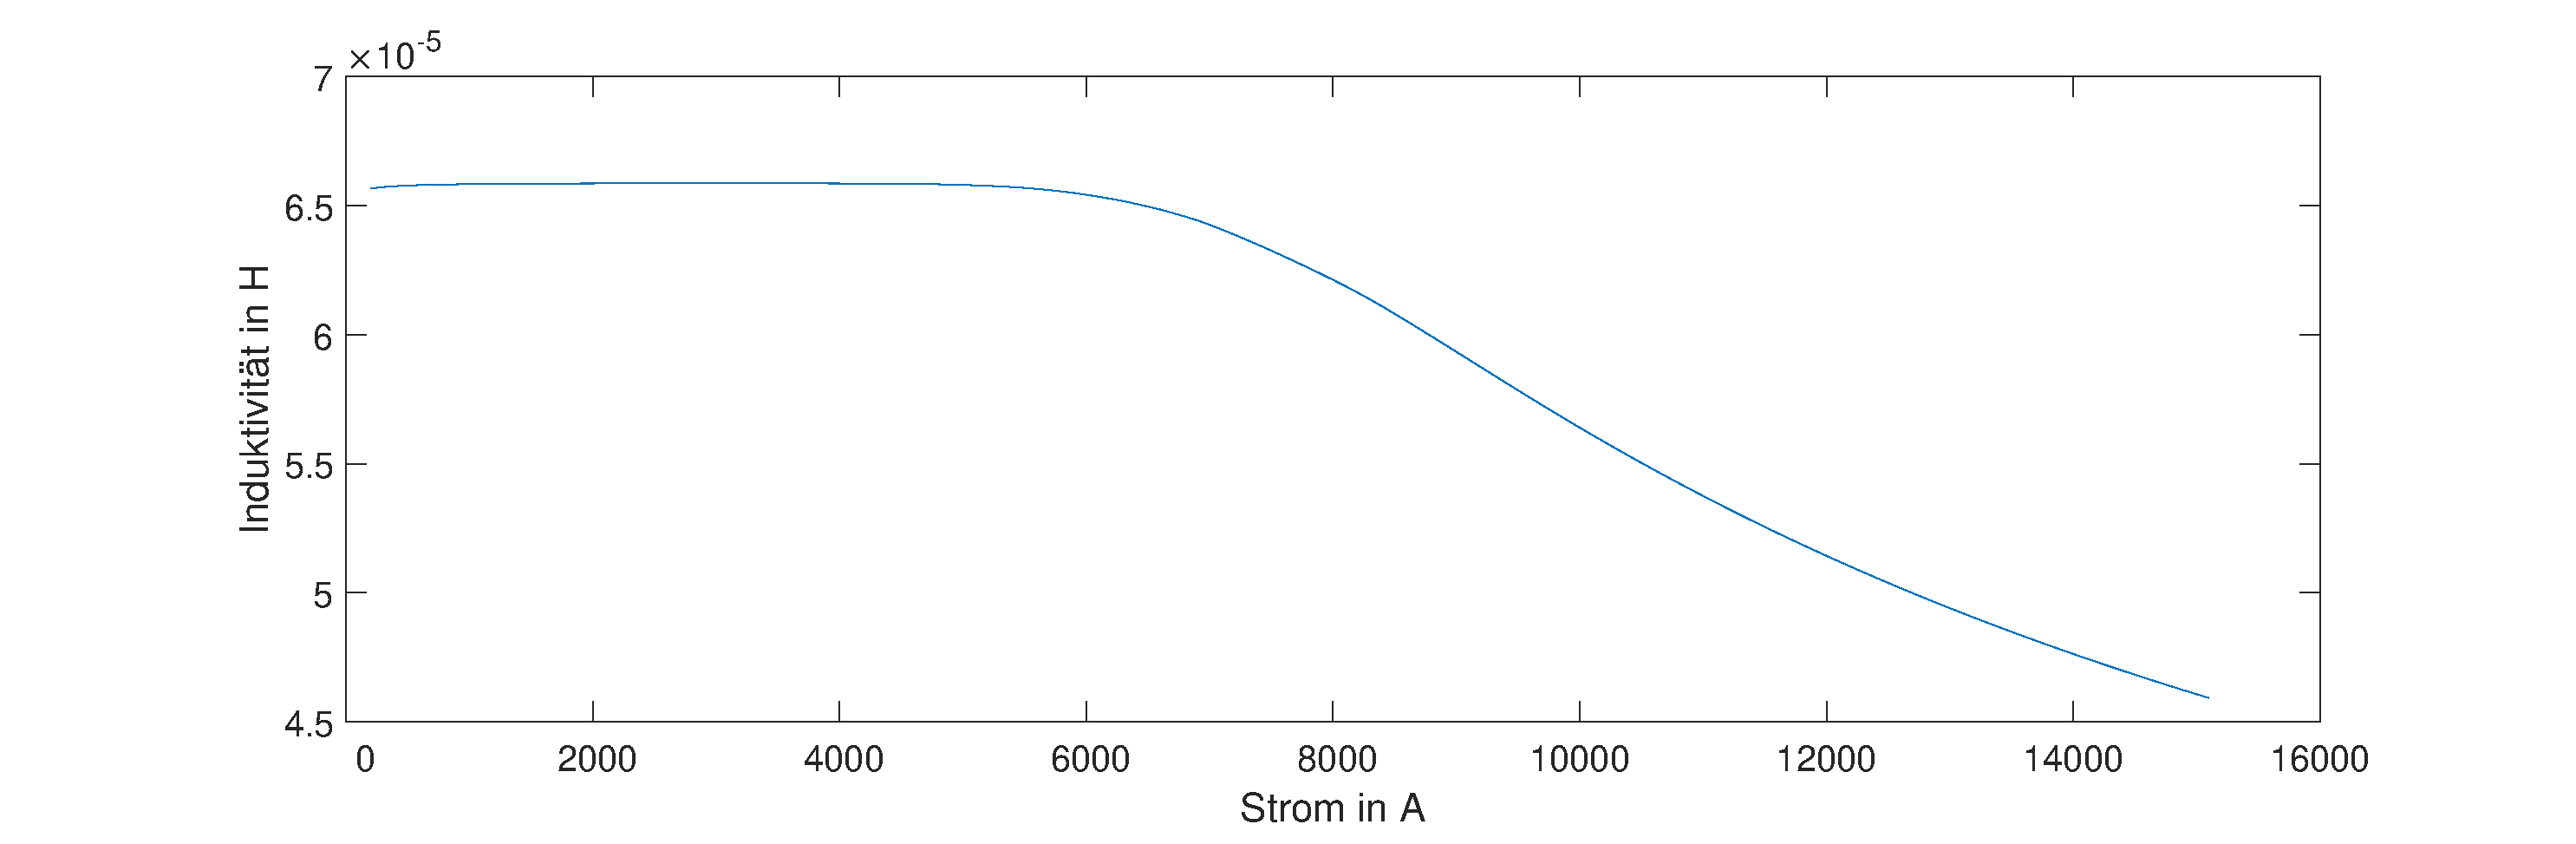
\includegraphics[width=\textwidth]{data/Ag8_3dplot}
	\caption{Induktivität in Abhängigkeit der Stromanregung}
	\label{fig:plot}
\end{figure}
	%%%%%%%%%%%%%%%%%%Fazit%%%%%%%%%%%%%%%%%%%%%%
	\chapter{Fazit}\label{sec:fazit}
%\addcontentsline{toc}{section}{Fazit}
Die erste Aufgabe ergab, dass sich die beiden Leiter des Koaxialkabels wie die Platten eines Plattenkondensators verhalten. Darüber hinaus ergibt sich, dass man durch Anfügen von weiteren Segmenten an die Schaltung eine Verkleinerung der Schwingfrequenz bewirkt.
Differentialgleichungen können häufig, wie sich in Aufgabe zwei zeigt, leichter im Frequenzbereich als im Zeitbereich gelöst werden. Die durch Lösen der Differentialgleichung analytisch berechneten Ergebnisse für Zeit- und Frequenzverhalten stimmen dabei mit der numerischen Simulation durch LTSpice überein.
Die Ergebnisse der dritten Aufgabe ergeben, dass sich die Feldlinien eines Kondensators in einem Simulationskäfig nicht nur senkrecht zu den Platten bewegen, sondern dass sich auch Randeffekte an den Enden der Kondensatorplatten ausbilden. Untersucht man unterschiedliche Randbedingungen zeigt sich, dass diese sowohl den Kapazitätswert des Kondensators, als auch die elektrischen Feldlinien beeinträchtigen. Die Wahl der Simulationsrandbedingungen kann also nicht willkürlich erfolgen.
	%%%%%%%%%%%%%%%%%%Anhang%%%%%%%%%%%%%%%%%%%%%
	\chapter{Anhang}\label{sec:anhang}
\lstset{ % Octave Settings
	language=Octave,
	extendedchars=true,
	basicstyle=\footnotesize,
	numbers=left,
	numberstyle=\tiny\color{gray},
	stepnumber=1,
	numbersep=10pt,
	showspaces=false,
	showstringspaces=false,
	tabsize=2,
	breaklines=true,
	frame=single,
	morecomment = [l][\itshape\color{blue}]{\%},
	captionpos=b,
	title=\lstname
}


\lstinputlisting{data/SIS.m}
\lstinputlisting{data/SkriptAg8_2.m}
\lstinputlisting{data/SkriptAg8_3d.m}



	%%%%%%%%%%%%%%%%%%%%%%%%%%%%%%%%%%%%%%%%%%%%%%%%%%%%%%%%%%%%%%%%%%%%%%%%%%%%%%%%%%%%%%%%%%%%%%%%%%
	
	%%%%%%%%%%%%%%%%%%%
	%Abbildungs- und Tabellenverzeichnis
	%%%%%%%%%%%%%%%%%%%
	\listoffigures % Abbildungsverzeichnis (captions in den Figuren werden als Referenz genommen)
	%\listoftables % Verzeichnis der Tabellen (captions in den Tabellen werden als Referenz genommen)
	
	%%%%%%%%%%%%%%%%%%%
	%Literaturverzeichnis an dieser Stelle
	%%%%%%%%%%%%%%%%%%%
	
	
\end{document}
